\section{Численные эксперименты}

\indent
\indent
В данной главе мы обсудим экспериментальную часть работы, начиная от
архитектуры программы и заканчивая обсуждением полученных результатов.



\subsection{Архитектура программы}

\indent
\indent
Основная часть программы, выполняющая обучение и тестирование модели
 состоит из стандартного для фреймворка \textit{pytorch} набора 
 взаимносвязанных компонент (классов). Перечислим их:


\begin{itemize}

	\item
	\textit{Module} --- описывает непосредственно вычислительный граф нейросети. 
	Здесь указаны параметры и количество всех слоев, описаны связи между ними.
	
	\item
	\textit{Dataset} --- позволяет итерироваться по набору данных и объединять их в 
	батчи для подачи на вход нейросети.
	
	\item
	\textit{Loss} --- вычисляет функцию ошибки/потери между предсказанными 
	моделью  и правильными значениями целевой переменной.
	
	\item
	\textit{Optimizer} --- совершает шаг градиентого спуска на заданное расстояние,
	которое определяется скоростью обучения \textit{(learning rate)}. А именно,
	изменяет веса модели так, чтобы уменьшить среднюю ошибку для очередного
	поданного на вход модели батча данных.
	
	\item
	\textit{Scheduler} --- изменяет скорость обучения модели \textit{(learning rate)}
	с течением времени по заданному правилу.
	
	\item
	\textit{Stopper} --- останавливает тренировку при выполнении заданного 
	условия, например, если в течение последних \textit{n} эпох не произошло
	увеличения точности модели хотя бы на $\epsilon$.
	
	\item
	\textit{MetricsCalculator} --- оценивает точность модели на некоторой размеченной
	подвыборке данных по заданным метрикам.
	
	\item
	\textit{TensorboardX}  --- система для визуального логирования обучения
	модели; позволяет строить графики изменения функции ошибки, метрик и
	выводить любые другие пользовательские изображения.
	
	\item
	\textit{Trainer} -- объединяет воедино компоненты, названные выше. Обучает
	модель эпоху за эпохой, с заданной частотой проверяет текущую точность
	на тестовом подмножестве данных. Останаливает тренировку по
	достижению некоторого критерия. Сохраняет промежуточные
	веса модели. Визуализирует процесс обучения.
 
 \end{itemize}


 \indent
 \indent
 Взаимосвязь между компонентами программы можно проследить на 
  рисунке \ref{tikzpicture: programm}.

\begin{figure}[h!]
    \begin{center}
   	    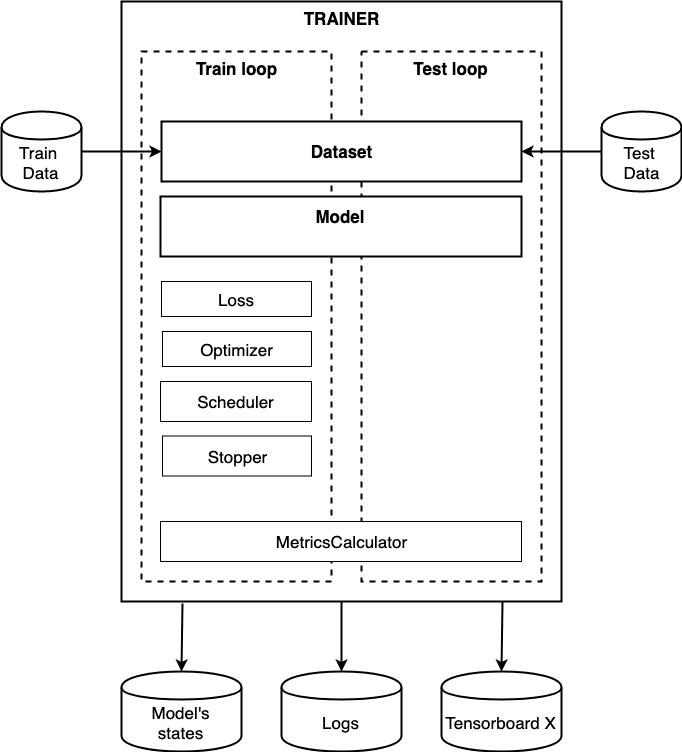
\includegraphics[width=0.95\linewidth]{Programm}
   	\end{center}
   	\caption{Структура программы для тренировки и обучения модели.}
   	\label{tikzpicture: programm}
\end{figure}



\subsection{Особенности реализации}
todo TTA



\subsection{Полученные результаты}
Картинка, графики метрик, confusion matrix



\subsection{Обсуждение результатов}


